\section{Développement firmware}
Dans cette section, nous allons décrire et expliquer le procédé de programmation du code qui a été implémenté dans le microcontrôleur PIC32MX130F256D.
Le processus de programmation du code dans le PIC32MX130F256D implique plusieurs étapes. Tout d'abord, il est nécessaire de disposer d'un environnement de développement intégré (IDE) adapté à ce microcontrôleur, ici, MPLAB X IDE, avec l'environnement Harmony permettant l'utilisation d'un configurateur graphiques pour les différentes libraires du PIC.

\subsection{Configuration des PINs dans Harmony}
{
	\begin{figure}[h]
		\centering
		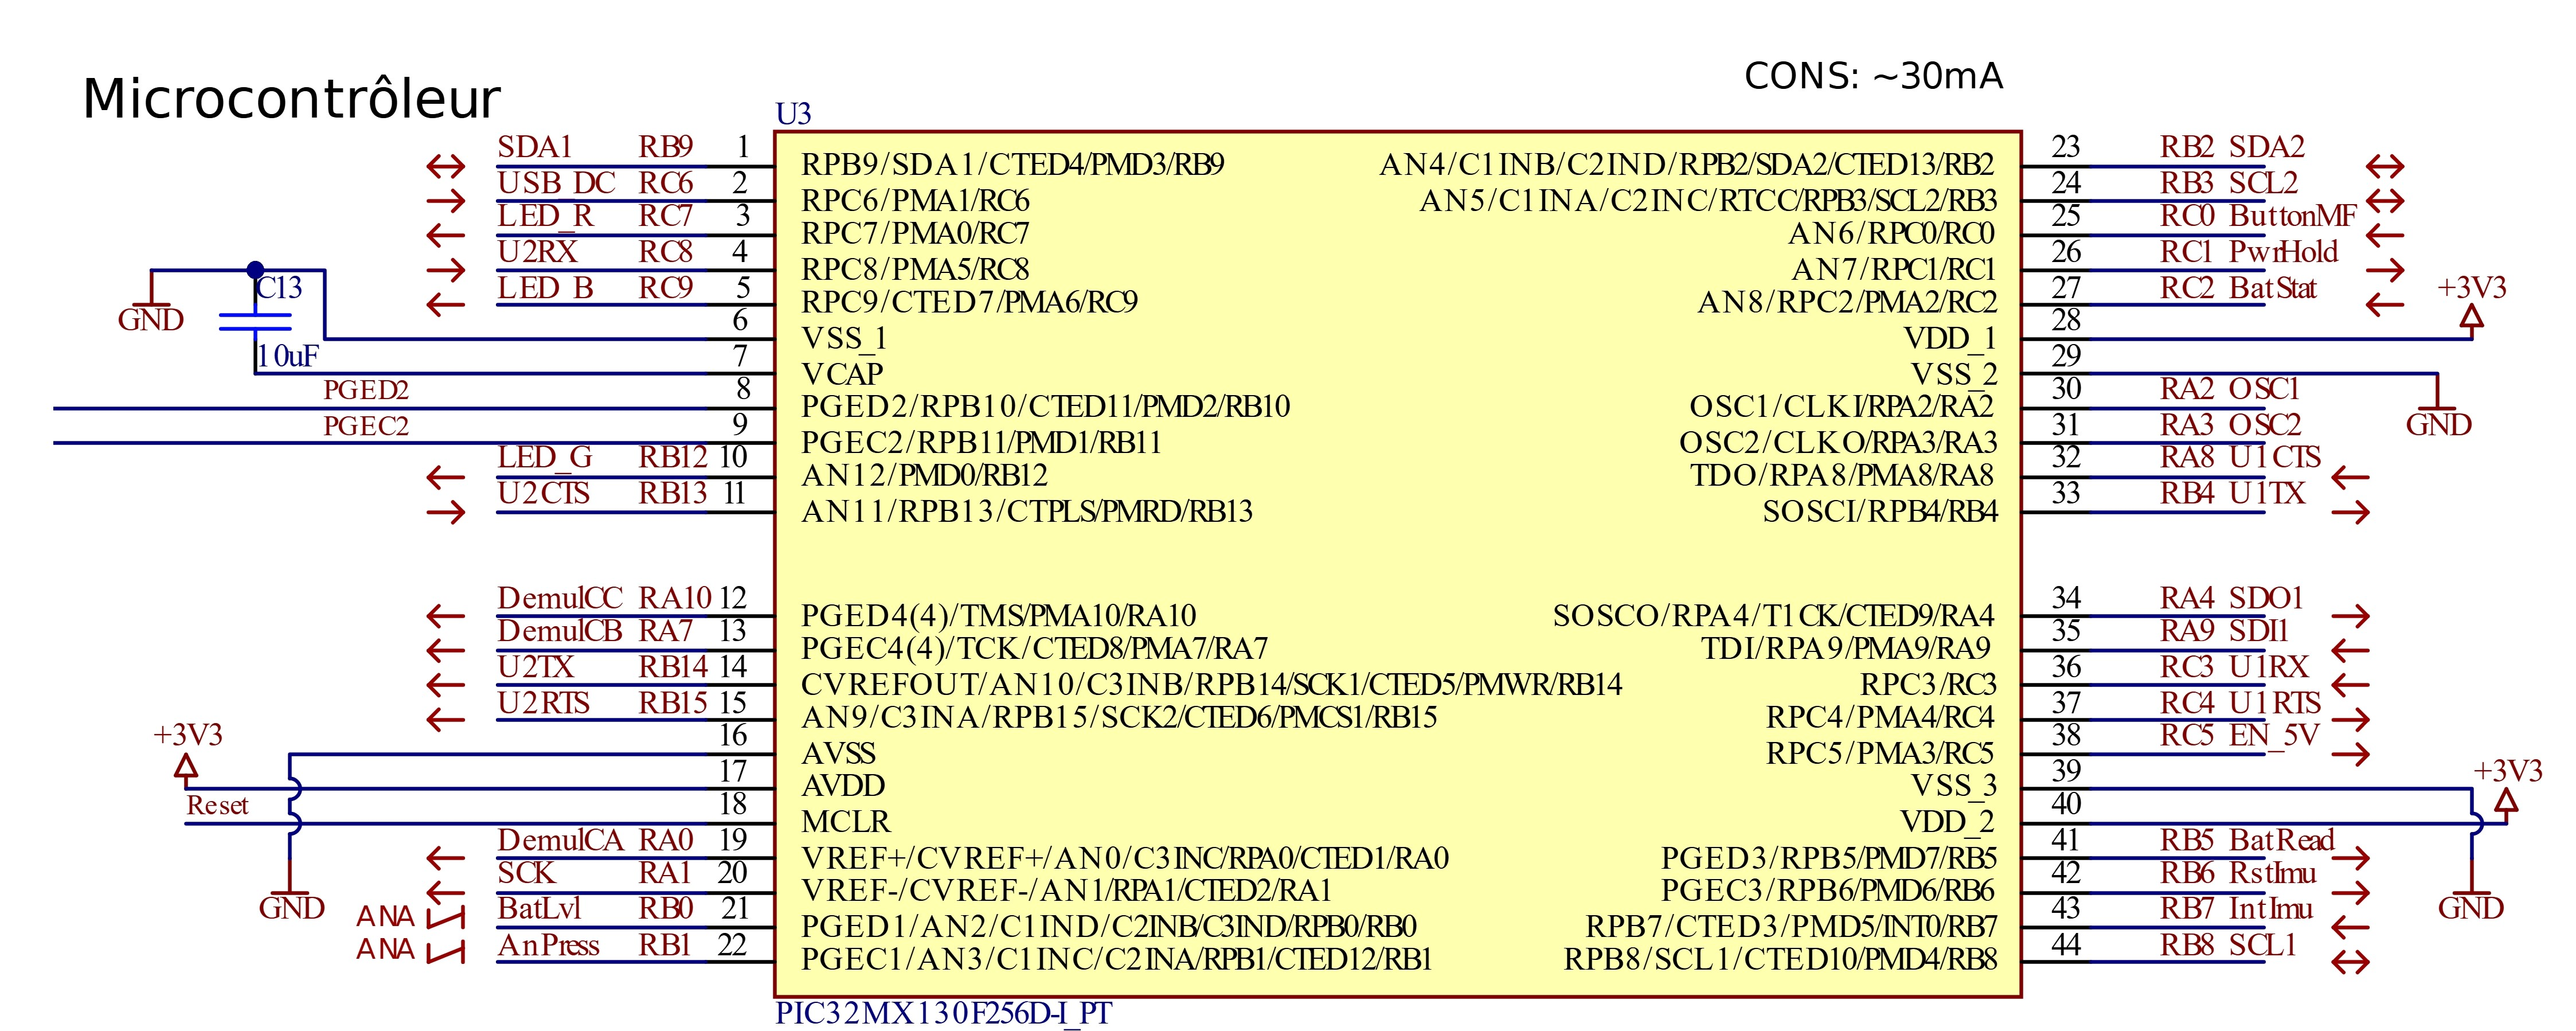
\includegraphics[width=.9\textwidth]{Figures/Dev-SOFT/MCU-Altium}
		\caption{Pinning réelles dans altium designer}
		\label{fig:mcu-altium}
	\end{figure}
	\begin{figure}[h]
		\centering
		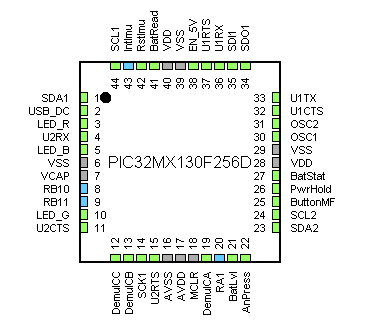
\includegraphics[width=0.5\textwidth]{Figures/Dev-SOFT/MCU-Harmony}
		\caption{Pinning dans Harmony}
		\label{fig:mcu-harmony}
	\end{figure}
	
	On peut voir que la PIN 20 (SCK) est en haute impédance dans harmony, tandis que la PIN14 qui était supposée être \textit{U2TX} est devenue SCK, ceci étant dû à une erreur : SCK n'est que valable sur la PIN14, il a donc fallut ajouter un fil extérieur pour router Pin14 à Pin20, sacrifiant ainsi la communication USB sur l'UART2, cette modification sera décrite ultérieurement.
	
	
}

\subsection{Configuration des périphériques dans Harmony}
{
	\subsubsection{Timers} 
	
	Deux timers seront utilisés, l'un pour mesurer des attentes en ms et l'autre moins rapide, pour les diverses actions du programmes, avec une interruptions chaque 10ms.
	\begin{table}[h]
		\centering
		\begin{tabular}{|l|l|}
			\hline
			Timer & Temps voulu \\
			\hline
			Timer 1 & 1ms \\
			\hline
			Timer 2 & 10ms \\
			\hline
		\end{tabular}
	\end{table}

	La clock du système a été accélérée a 48MHz, cela dans le but d'accéléré le système dans sa globalité, sachant qu'il y a beaucoup de communication qui nécessite des opérations rapides, que ce soit dans la préparation des buffers ou les différents calculs.
	
	\begin{figure}[h]
		\centering
		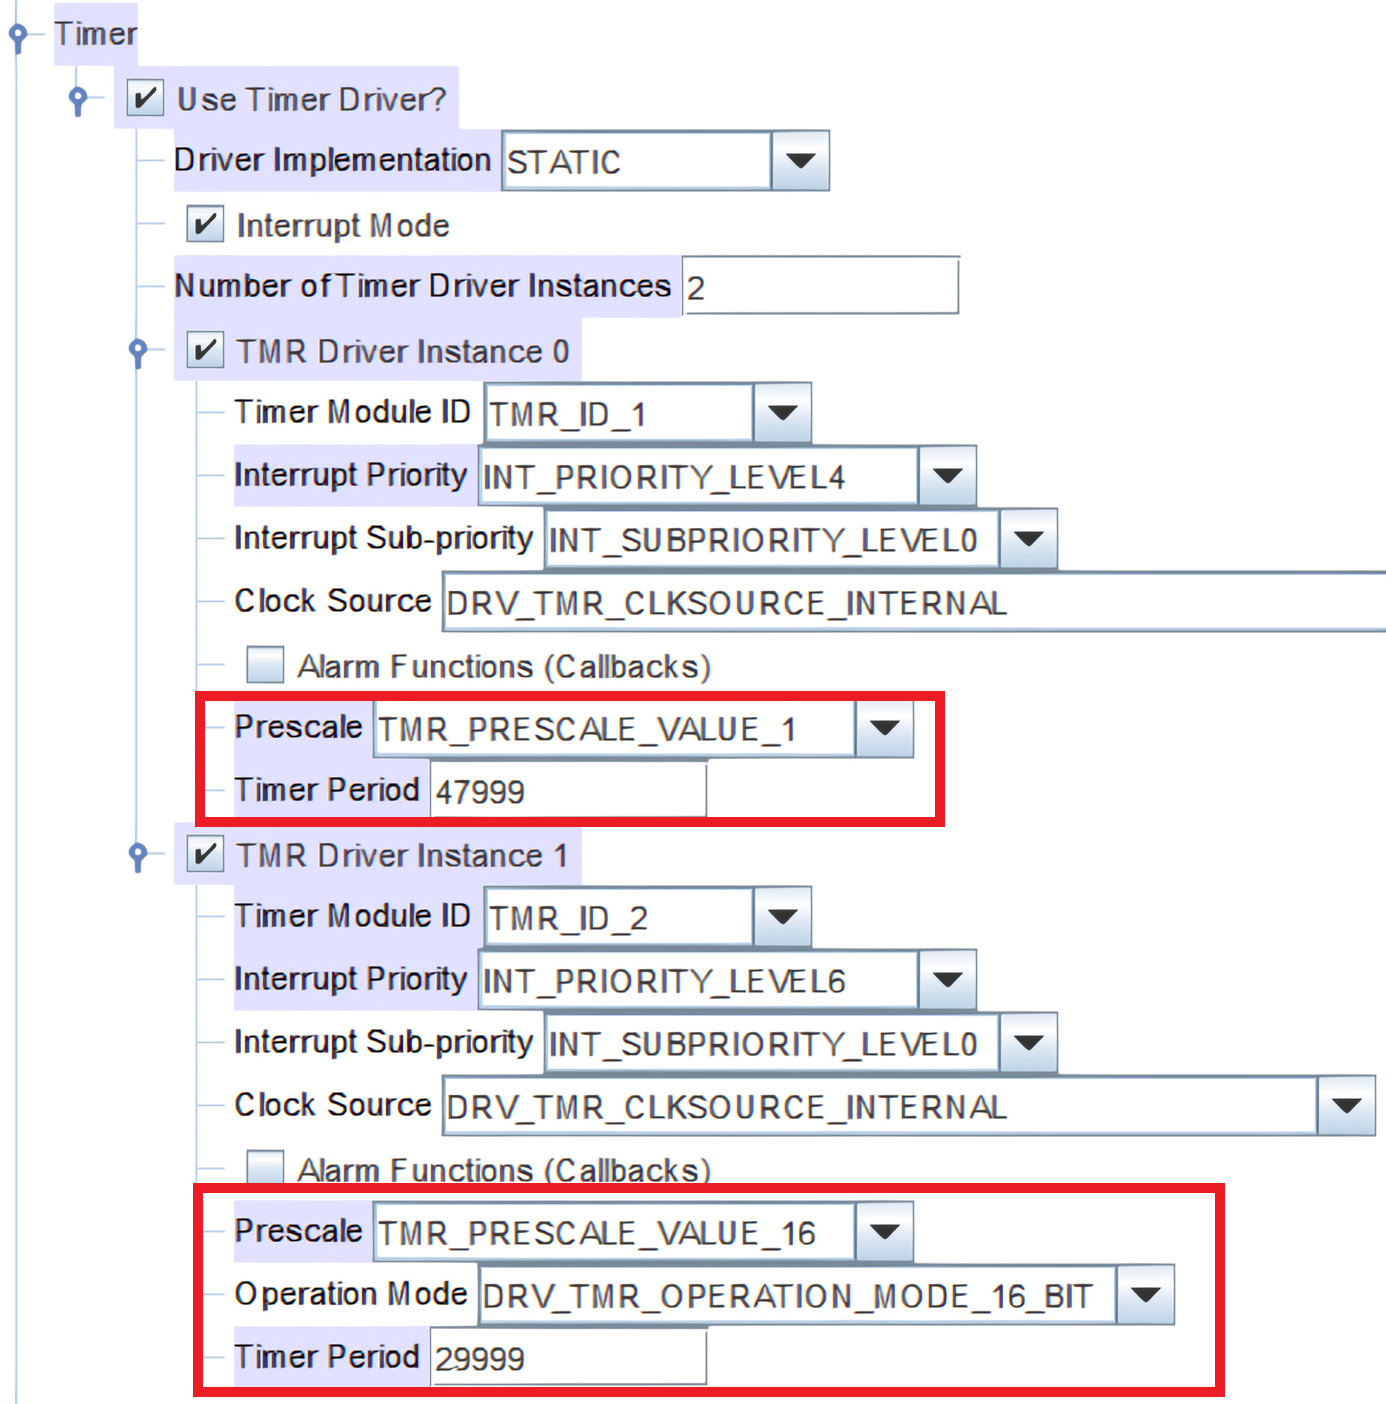
\includegraphics[width=0.55\linewidth]{Figures/Dev-SOFT/Timer_config}
		\caption{Configuration dans harmony}
		\label{fig:timerconfig}
	\end{figure}

	\begin{figure}[h]
		\centering
		\begin{subfigure}[b]{0.45\textwidth}
			\centering
			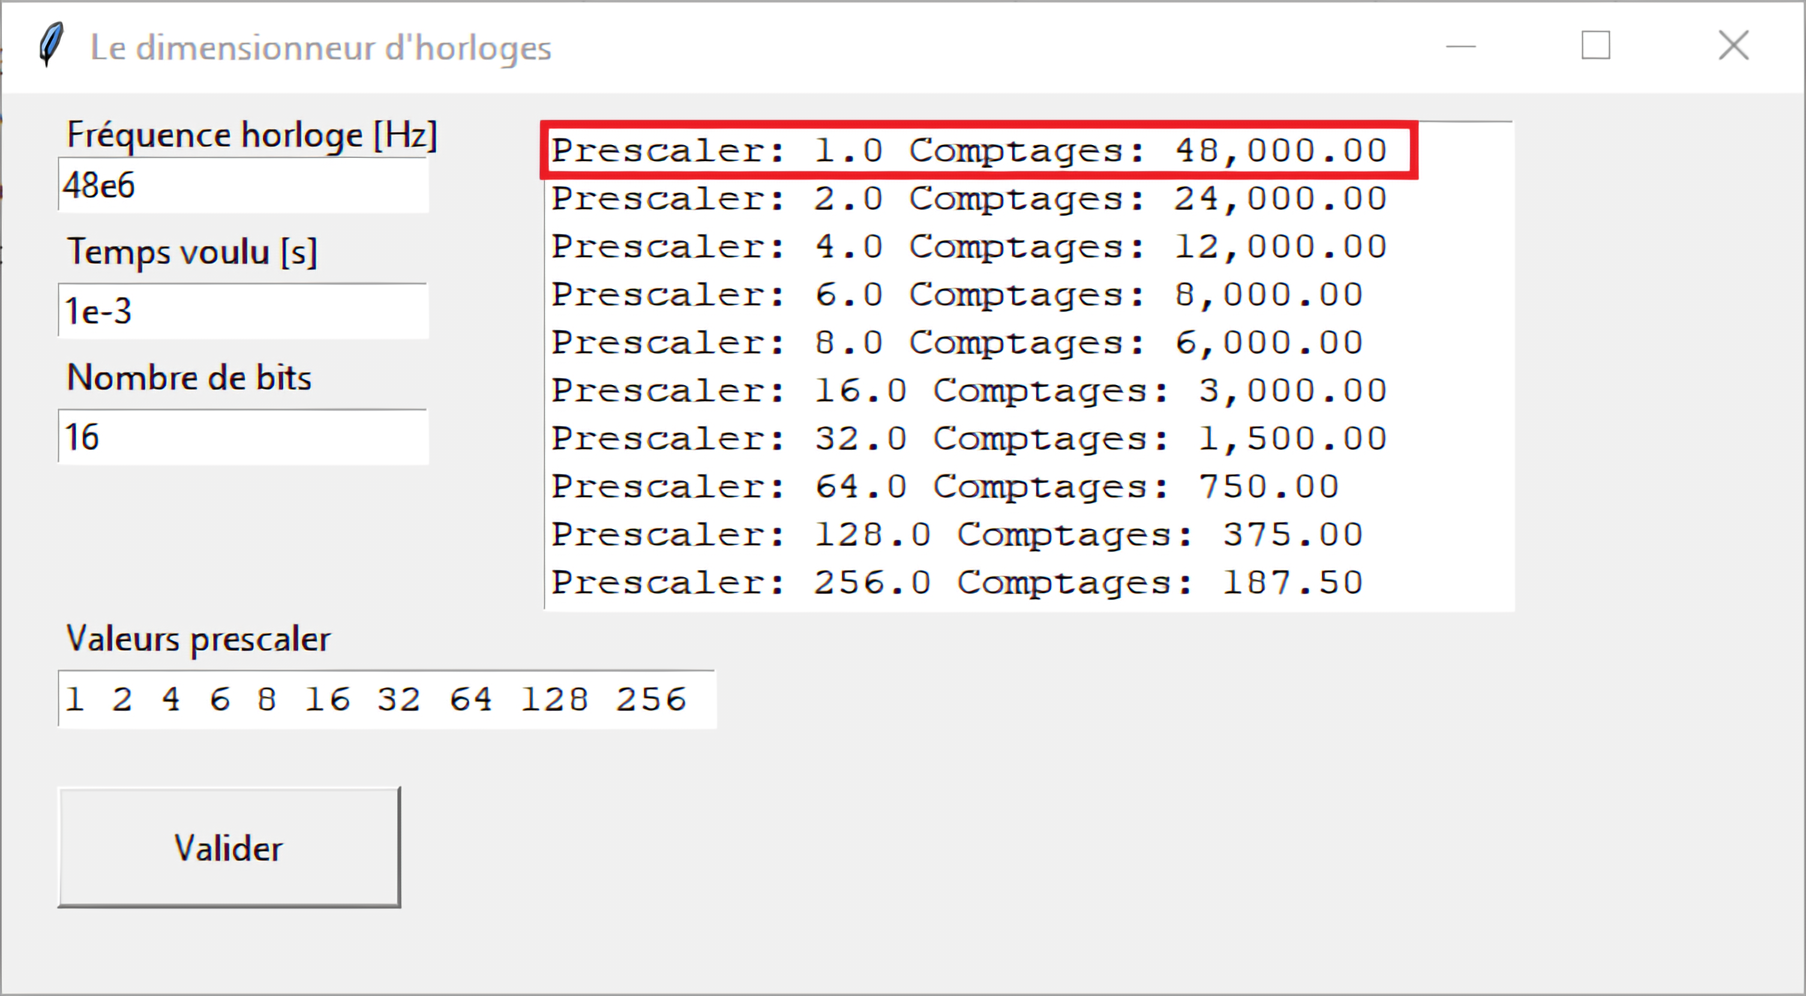
\includegraphics[width=\textwidth]{Figures/Dev-SOFT/Timer1ms}
			\caption{Timer 1, Dimensionnement pour 1ms}
			\label{fig:timer1ms}
		\end{subfigure}
		\hfill
		\begin{subfigure}[b]{0.45\textwidth}
			\centering
			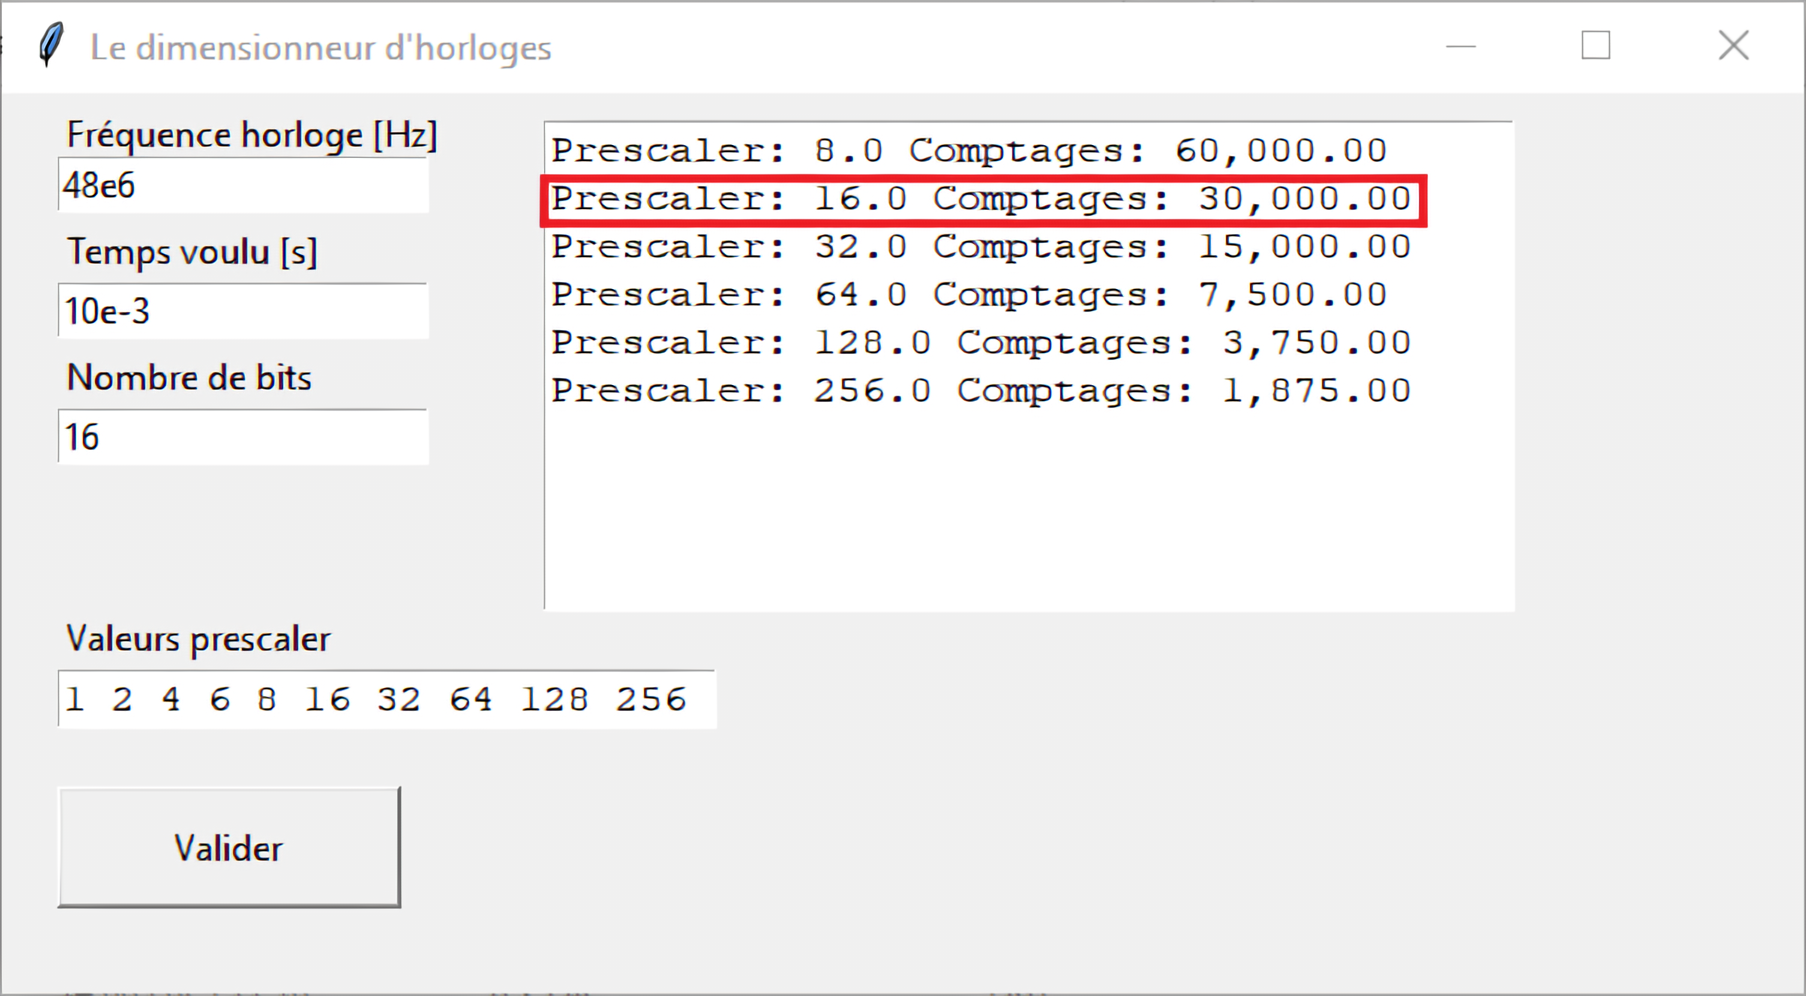
\includegraphics[width=\textwidth]{Figures/Dev-SOFT/Timer10ms}
			\caption{Timer 2, Dimensionnement pour 10ms}
			\label{fig:timer10ms}
		\end{subfigure}
		\hfill
		\caption{Application timer développée par l'auteur}
		\label{fig:appTimer}
	\end{figure}

	\clearpage

	\subsubsection{USART} 
	J'ai décidé de configurer une communication série dans le but  de vérifier mes données de mesures en temps réelles, simplifiant ainsi le debuggage. Pour se faire, j'ai décidé d'utiliser le périphériques UART1 prévu à la base pour le slot mikroe. Je viendrais ensuite me connecter avec un module USB-to-TTL externe pour lire les données via Putty sur mon ordinateur portable.
	
	\begin{figure}[h]
		\centering
		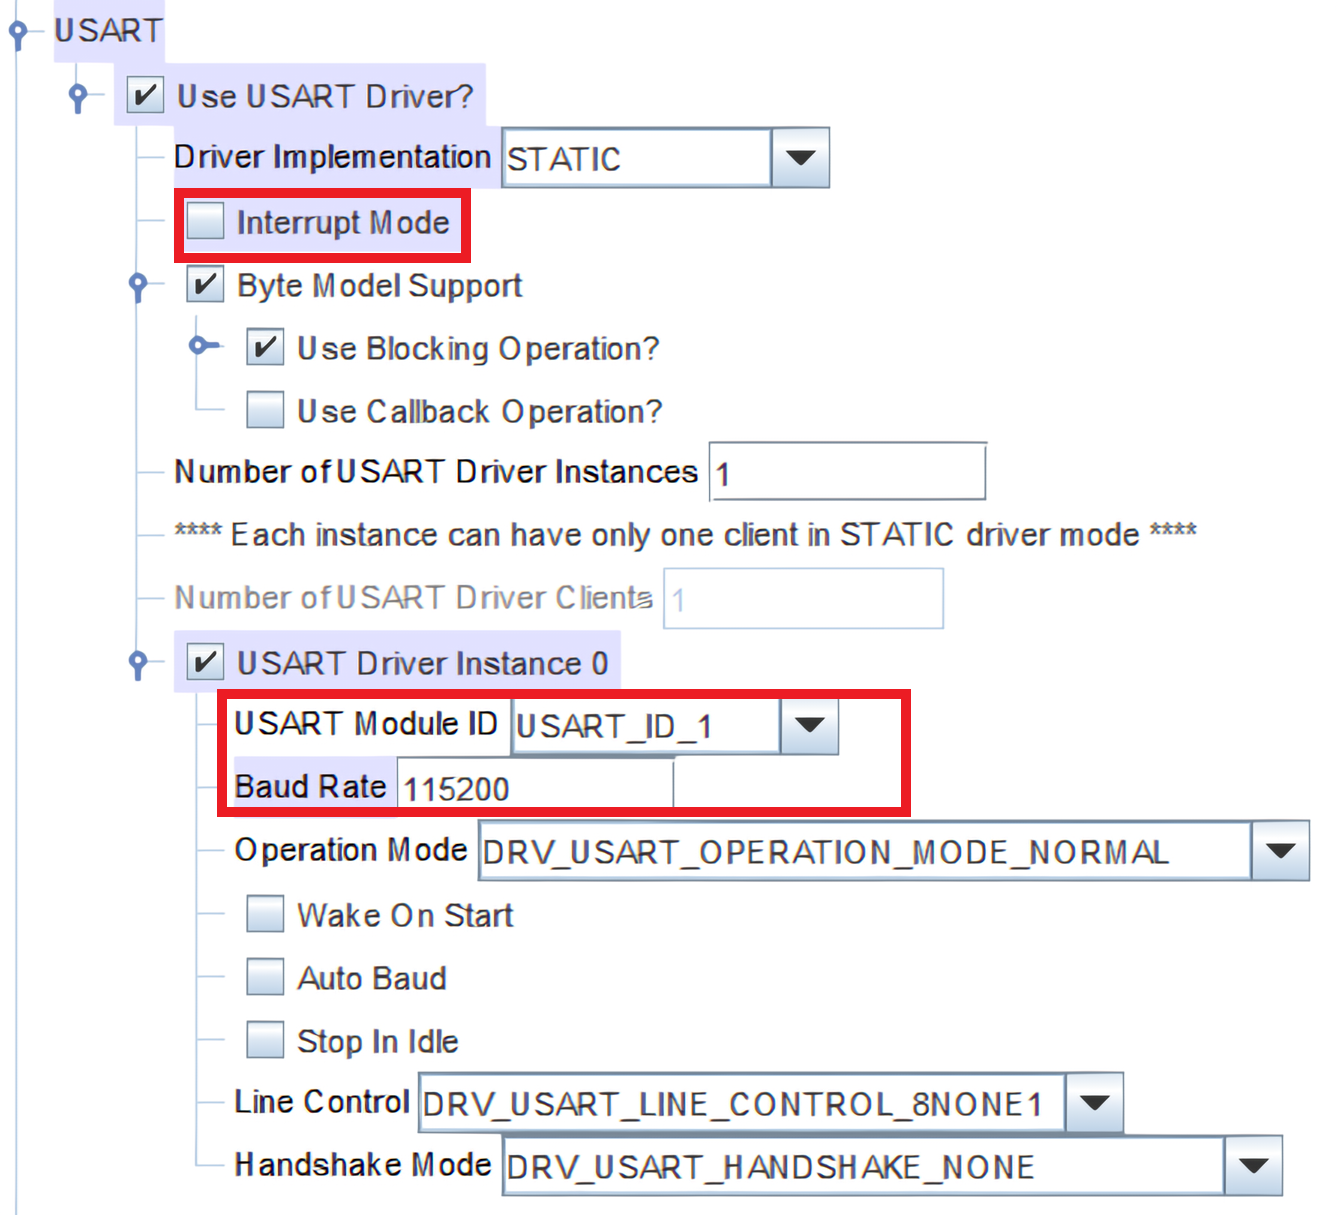
\includegraphics[width=0.7\linewidth]{Figures/Dev-SOFT/ConfigUart}
		\caption{Configuration UART}
		\label{fig:configuart}
	\end{figure}
	
	
	On peut constater sur la figure \ref{fig:configuart} que l'UART est configuré sans interruption a un bauderate de 115200.

	\subsubsection{Carte SD - SPI} 
	{
	J'ai optimisé l'utilisation du SPI en choisissant une fréquence de 5 MHz afin de minimiser le temps d'exécution sur le microcontrôleur, sachant que les opérations FAT nécessitent de nombreuses trames. Cependant, j'ai rencontré un problème lié à la clock du SPI. Étant donné la vitesse élevée et les modifications que j'ai dû effectuer, la clock interfère avec le FTDI inutilement, et un fil relie SCK et U2TX, créant ainsi une inductance parasite. Pour résoudre ce problème, j'ai dû ajouter un condensateur de \textbf{33pF} entre SCK et GND, pour stabiliser la communication. Voir la configuration harmony de la carte SD sur la figure \ref{fig:configsdspi}.
	\clearpage
	\begin{figure}[h]
		\centering
		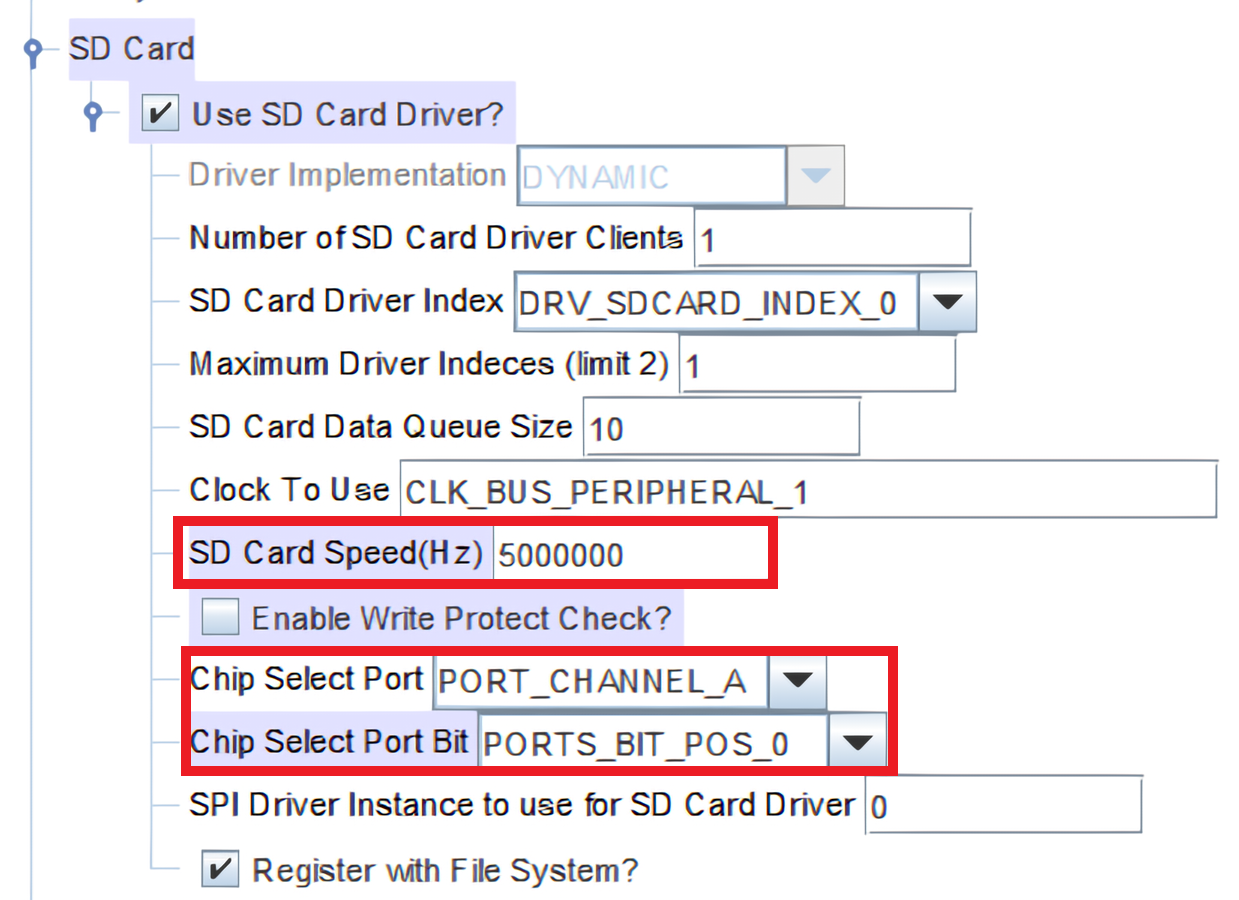
\includegraphics[width=0.7\linewidth]{Figures/Dev-SOFT/ConfigSD_SPI}
		\caption{Configuration du SPI}
		\label{fig:configsdspi}
	\end{figure}
	}

	\subsection{Code}
	Je vais dans cette section décrire le code du projet. Voici la hiérarchie des fichier du projet :
	\begin{figure}[h]
		\centering
		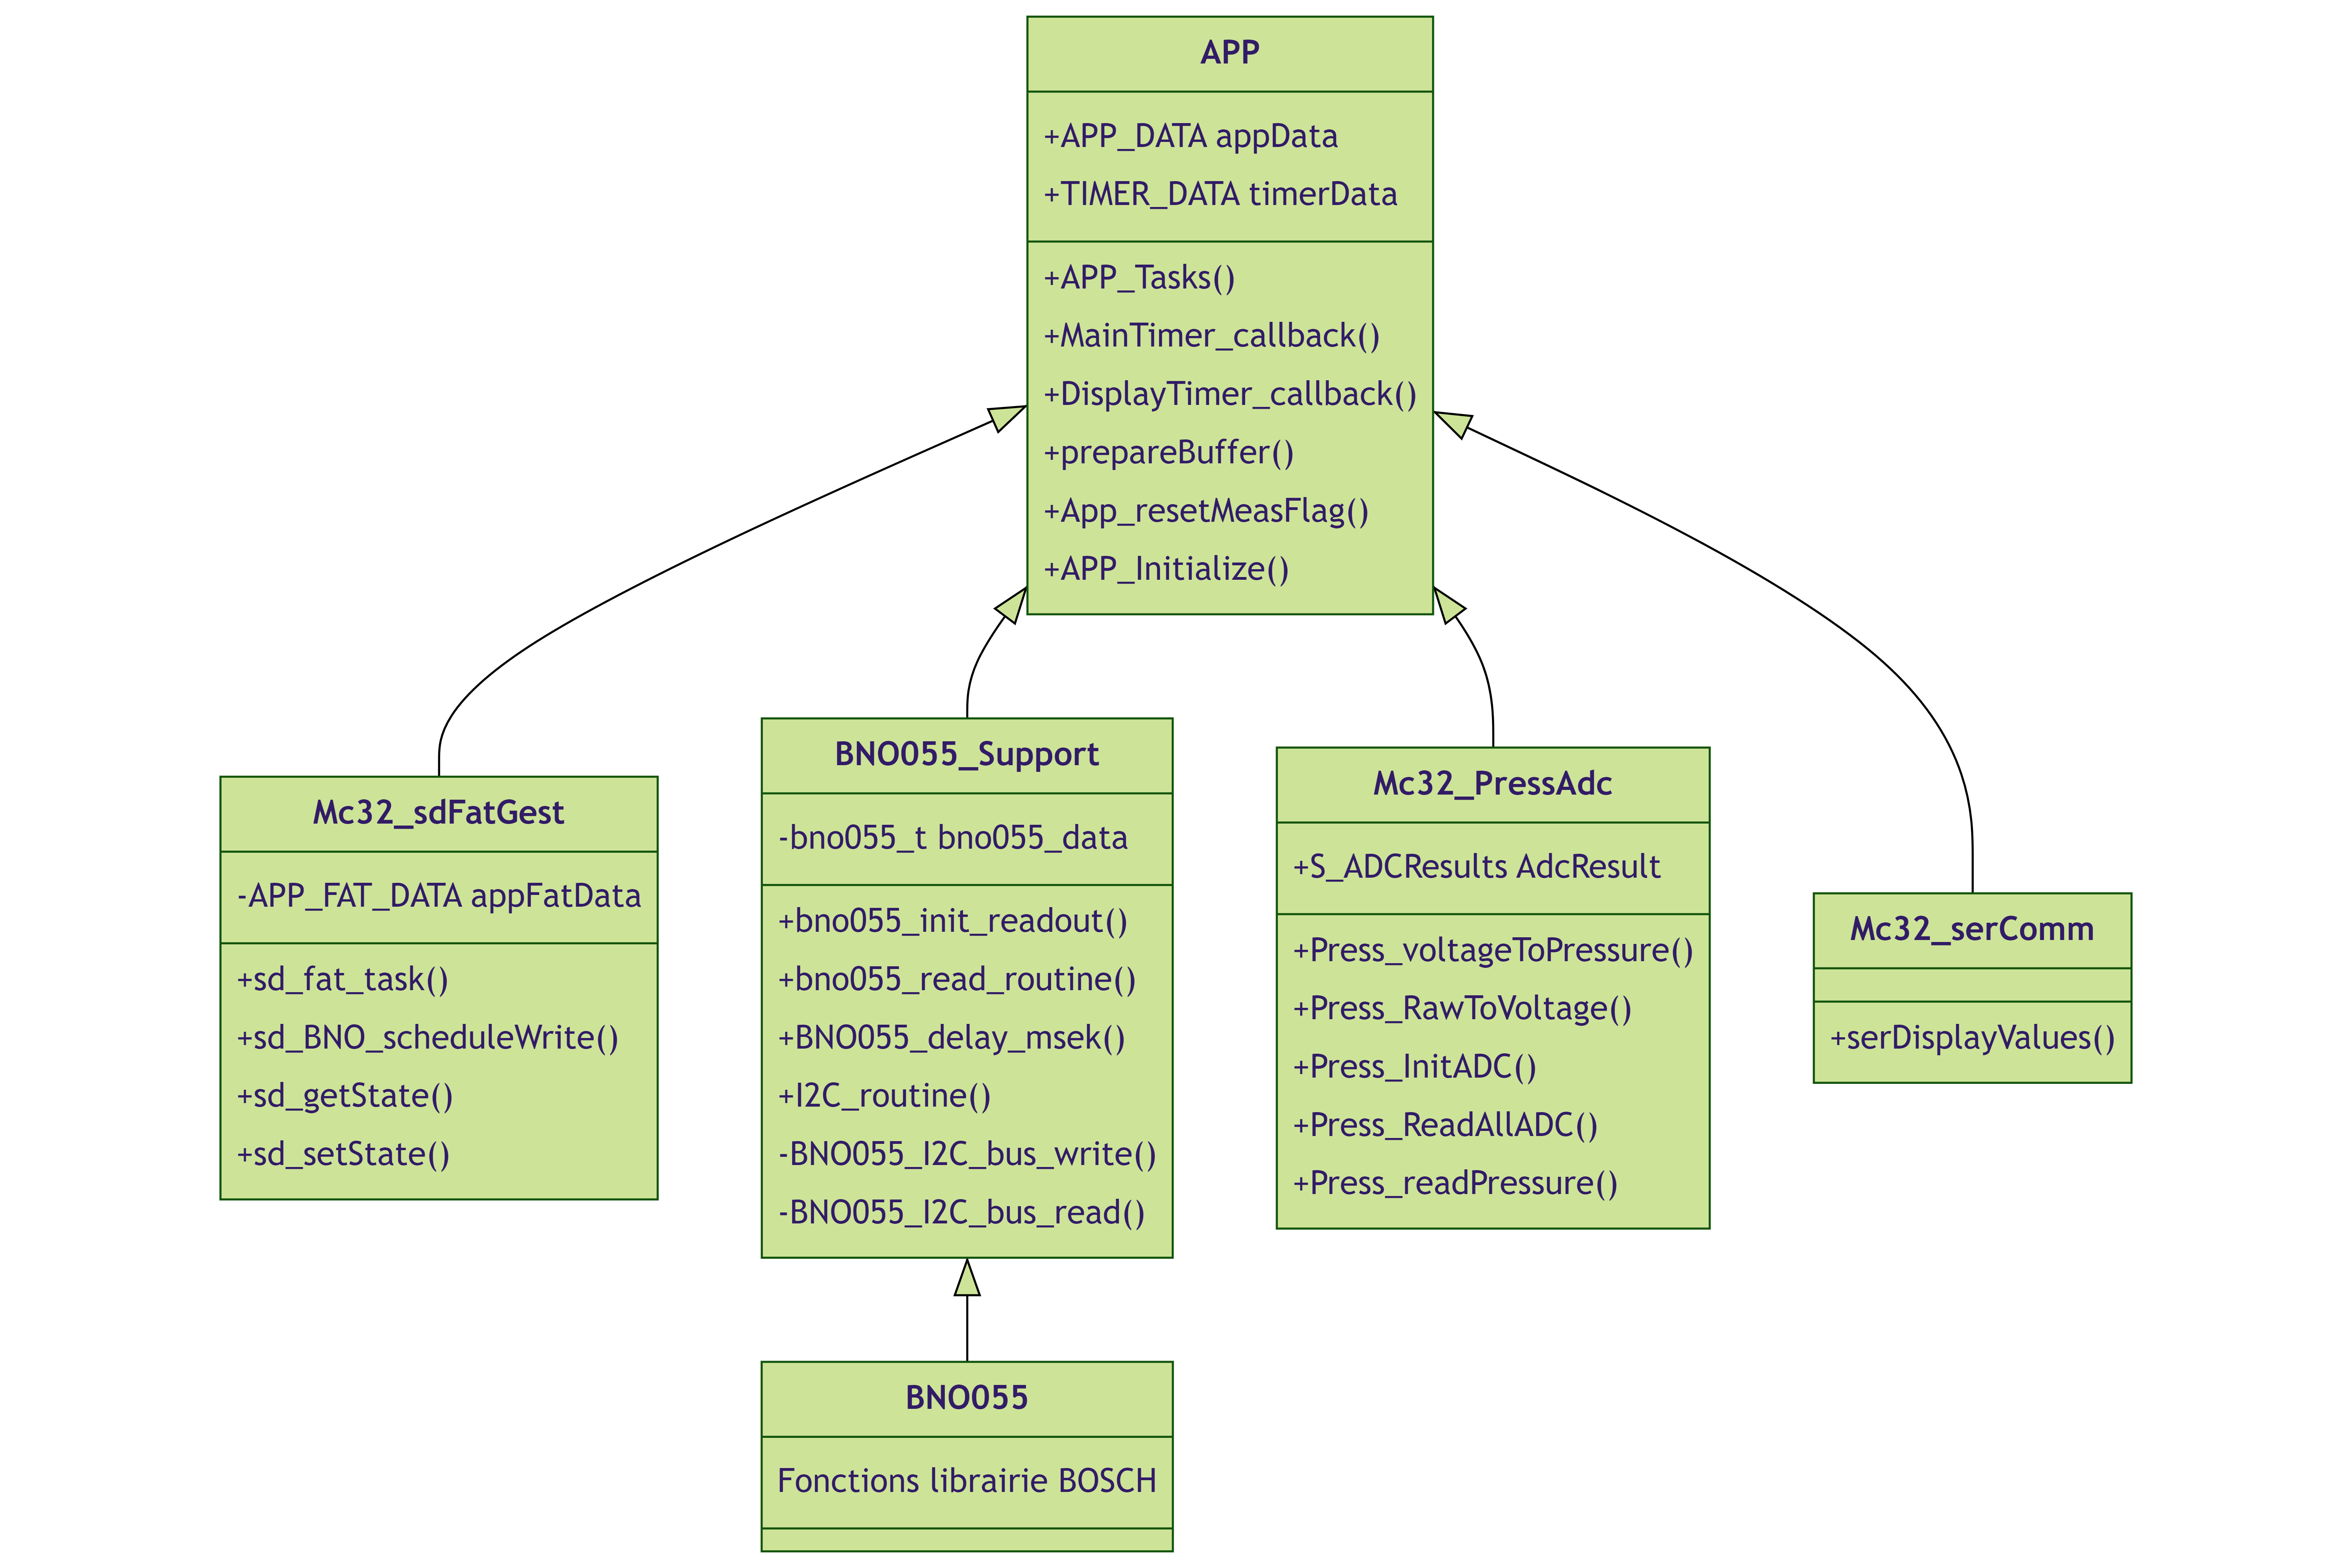
\includegraphics[width=0.725\linewidth]{Figures/Dev-SOFT/ClassesCode}
		\caption{Hiérarchie des fichiers du projet}
		\label{fig:classescode}
	\end{figure}
	
	\clearpage	
	
	\subsubsection{Callbacks}
	{
	Chacun des timers appellent dans leur interruption une fonction appartenante au fichier \textit{app.c} qui contient les actions définies pour chaque lapse de temps fixés. On peut visualiser cela sur le diagramme de la figure \ref{fig:callbacks}.
	
	\begin{figure}[h!]
		\centering
		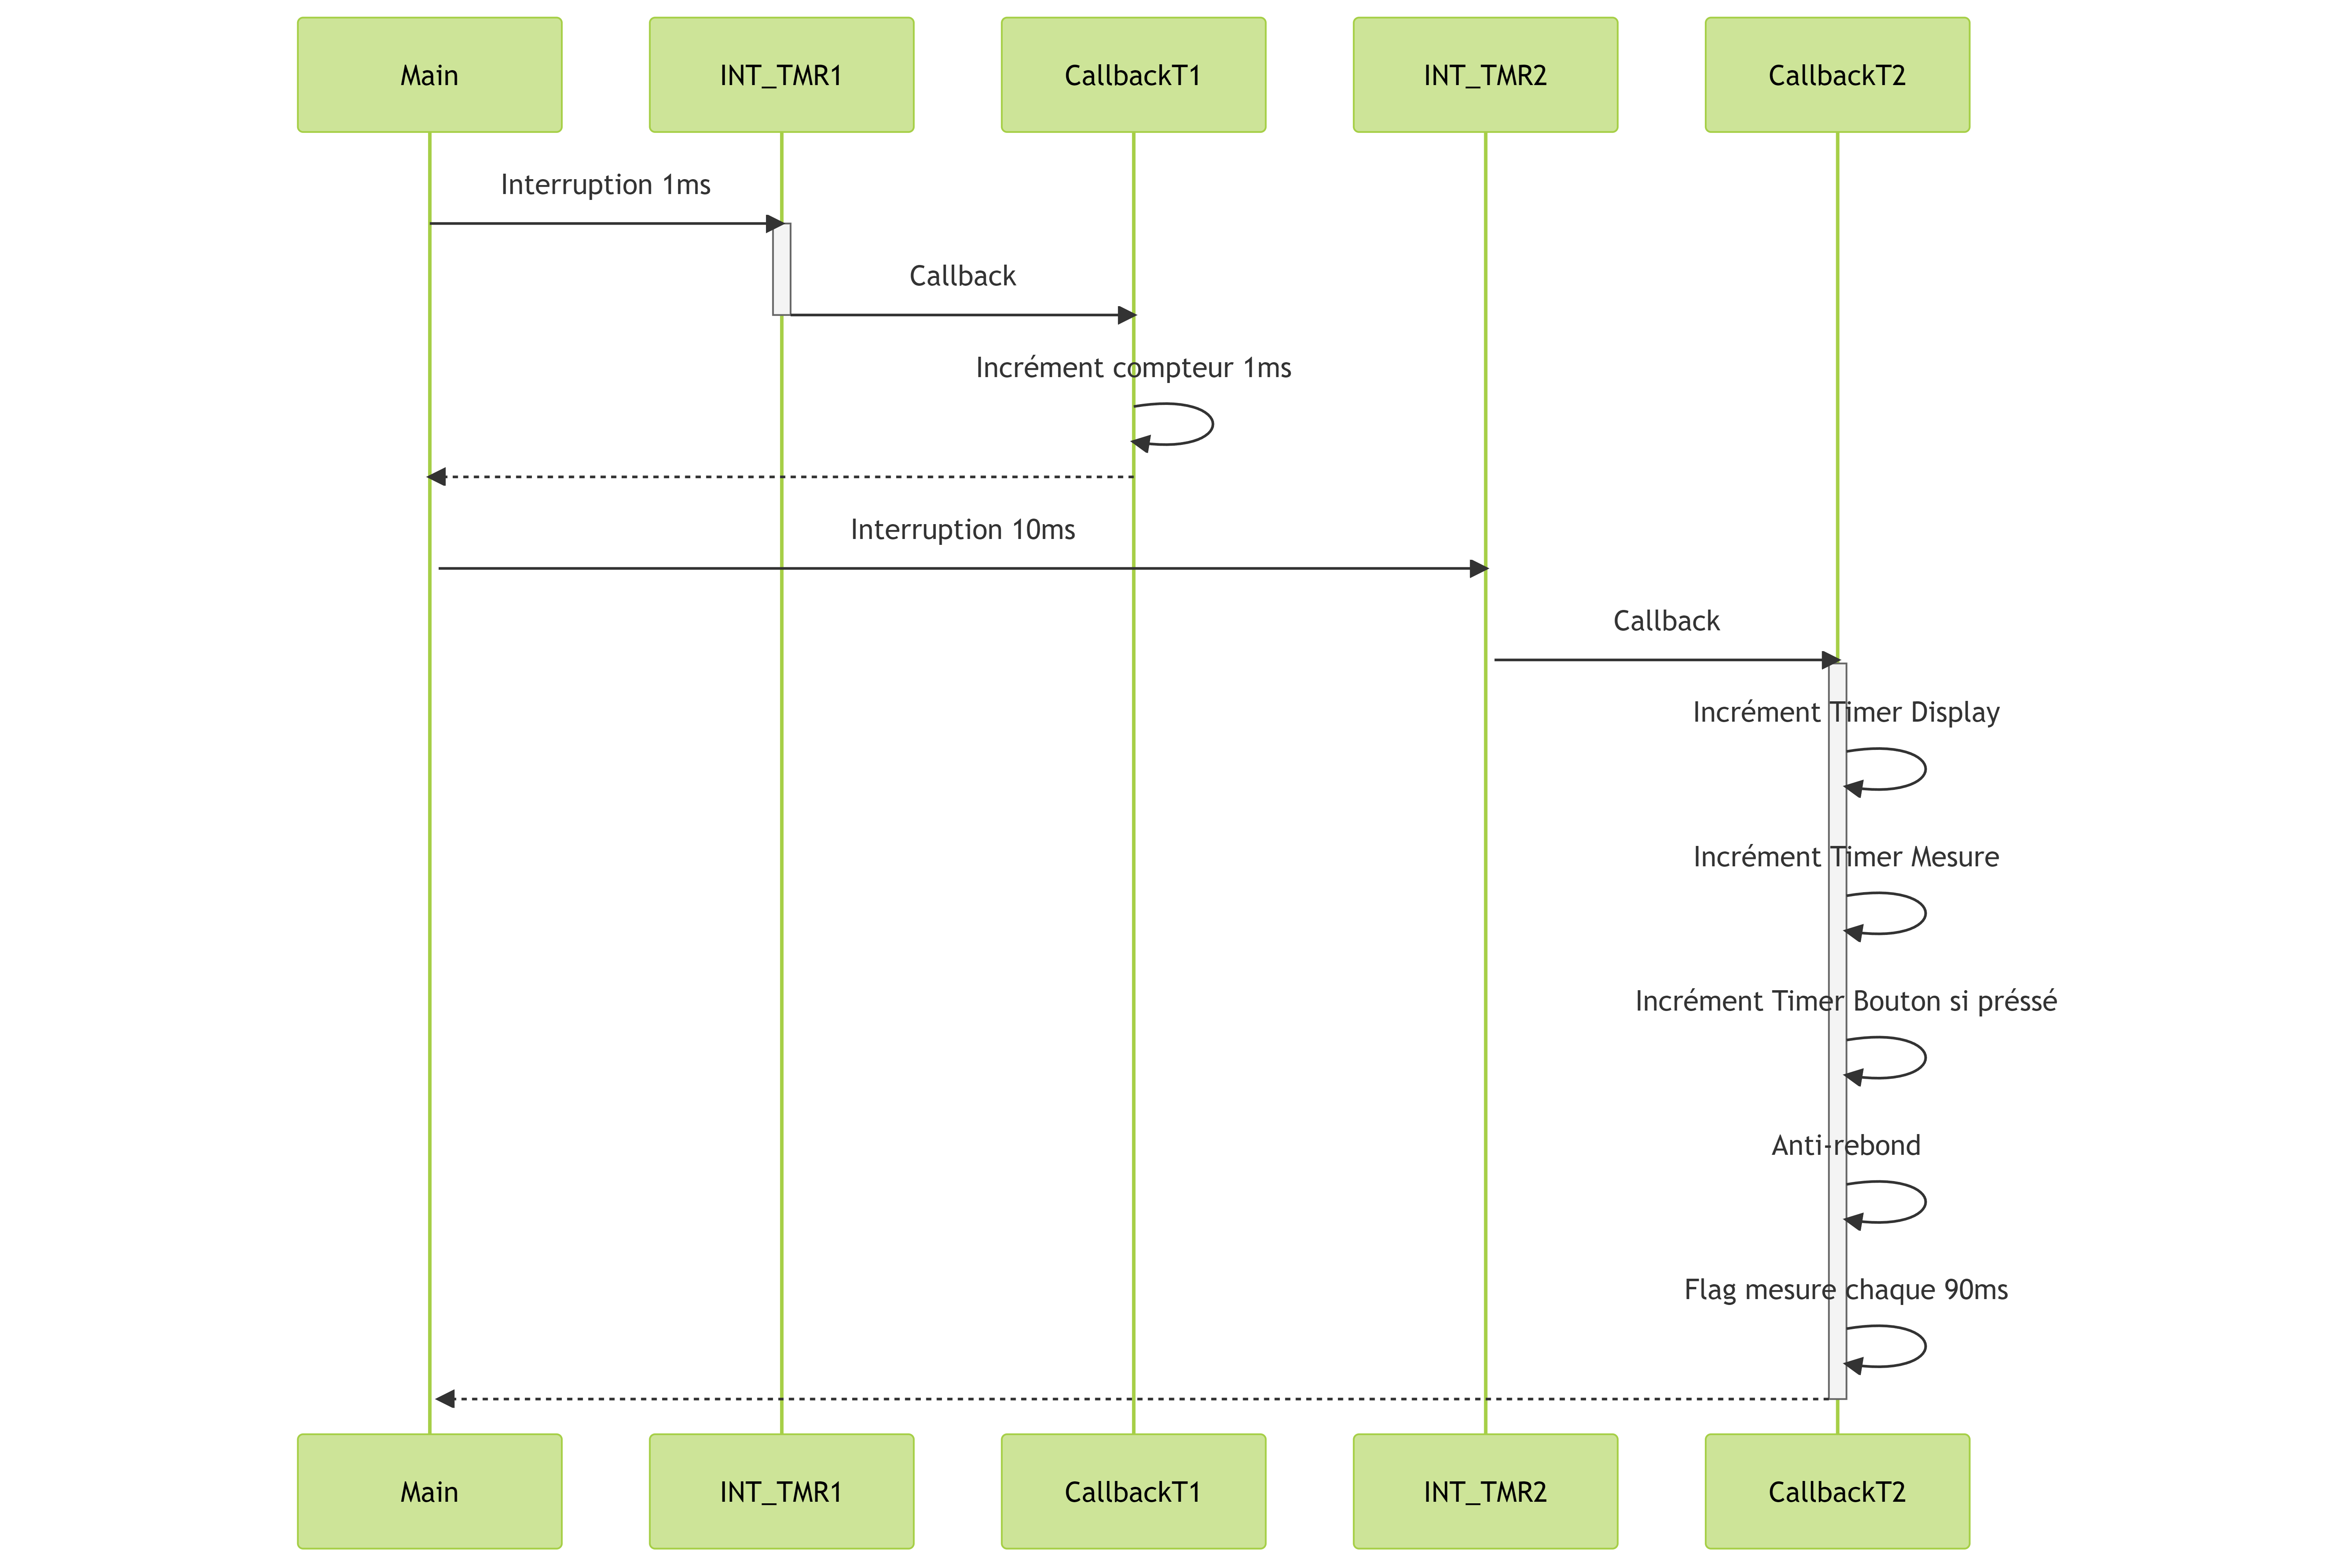
\includegraphics[width=.9\textwidth]{Figures/Dev-SOFT/Callbacks}
		\caption{Interactions des interruptions et des callbacks}
		\label{fig:callbacks}
	\end{figure}

	Les callbacks en C offrent flexibilité, extensibilité et réutilisabilité. Ils permettent d'ajuster dynamiquement le comportement du programme, d'étendre les fonctionnalités et de réutiliser le code. Les callbacks favorisent également l'encapsulation et la personnalisation, améliorant ainsi la modularité et la maintenance du code.	
	}
	
	\clearpage
	\subsubsection{Centrale inertielle BNO055}
	Pour ce qui est de la centrale inertielle BNO055, j'ai utilisé la libraire de BOSCH \footnote{\href{https://github.com/BoschSensortec/BNO055_driver}{Librairie du fabricant}}; La configurer pour du 32bits, créer les fonctions bas-niveau (i2c) et faire le liens avec la libraire BOSCH. Le tout dans le fichier BNO055\_support.c.
	
	Pour faire le lien entre la librairie haut-niveau et bas-niveau, j'ai utilisé un pointeur de fonction présent dans la structure de donnée du BNO :
	
\begin{lstlisting}[frame=single, language=C, caption={Code lien pointeur de fonction}, captionpos=b]
s8 I2C_routine(void)
{
	bno055.bus_write = BNO055_I2C_bus_write;
	bno055.bus_read = BNO055_I2C_bus_read;
	bno055.delay_msec = BNO055_delay_msek;
	bno055.dev_addr = BNO055_I2C_ADDR1;
	return BNO055_INIT_VALUE;
}
\end{lstlisting}

	Voici le code une écriture sur le BNO055 par I2C :
\begin{lstlisting}[frame=single, language=C, caption={Code écriture au BNO055}, captionpos=b, breaklines=true]
s8 BNO055_I2C_bus_write(u8 dev_addr, u8 reg_addr, u8 *reg_data, u8 cnt)
{
	s8 BNO055_iERROR = BNO055_INIT_VALUE;
	u8 array[I2C_BUFFER_LEN];
	u8 stringpos = BNO055_INIT_VALUE;
	array[BNO055_INIT_VALUE] = reg_addr;
	
	i2c_start();
	BNO055_iERROR = i2c_write(dev_addr<<1);
	
	for (stringpos = BNO055_INIT_VALUE; stringpos < (cnt+BNO055_I2C_BUS_WRITE_ARRAY_INDEX); stringpos++)
	{
		BNO055_iERROR = i2c_write(array[stringpos]);
		array[stringpos + BNO055_I2C_BUS_WRITE_ARRAY_INDEX] = *(reg_data + stringpos);
	}
	
	i2c_stop();
	if(BNO055_iERROR-1 != 0)
		BNO055_iERROR = -1;
	else
		BNO055_iERROR = 0;
	return (s8)(BNO055_iERROR);
}
\end{lstlisting}
	Pour ce qui est de l'utilisation de la libraire haut-niveau bno055\_support, voici la préparation et la lecture des données : 
	
	\begin{lstlisting}[frame=single, language=C, caption={Code lecture des données par la librairie}, captionpos=b, breaklines=true]
/* BNO055 Read all important info routine */
bno055_local_data.comres = bno055_read_routine(&bno055_local_data);
/* Delta time */
bno055_local_data.d_time = timerData.TmrMeas - timerData.ltime;
/* Pressure measure */
bno055_local_data.pressure = Press_readPressure();
/* Flag measure value */
bno055_local_data.flagImportantMeas = flagMeas;
	\end{lstlisting}

	\subsubsection{Carte SD}
	La carte SD sa communication fonctionne sous forme d'une machine d'état non-bloquante, permettant ainsi de s'adapter aux situations de la carte sans bloquer le système pour autant.
	
	\begin{figure}[h]
		\centering
		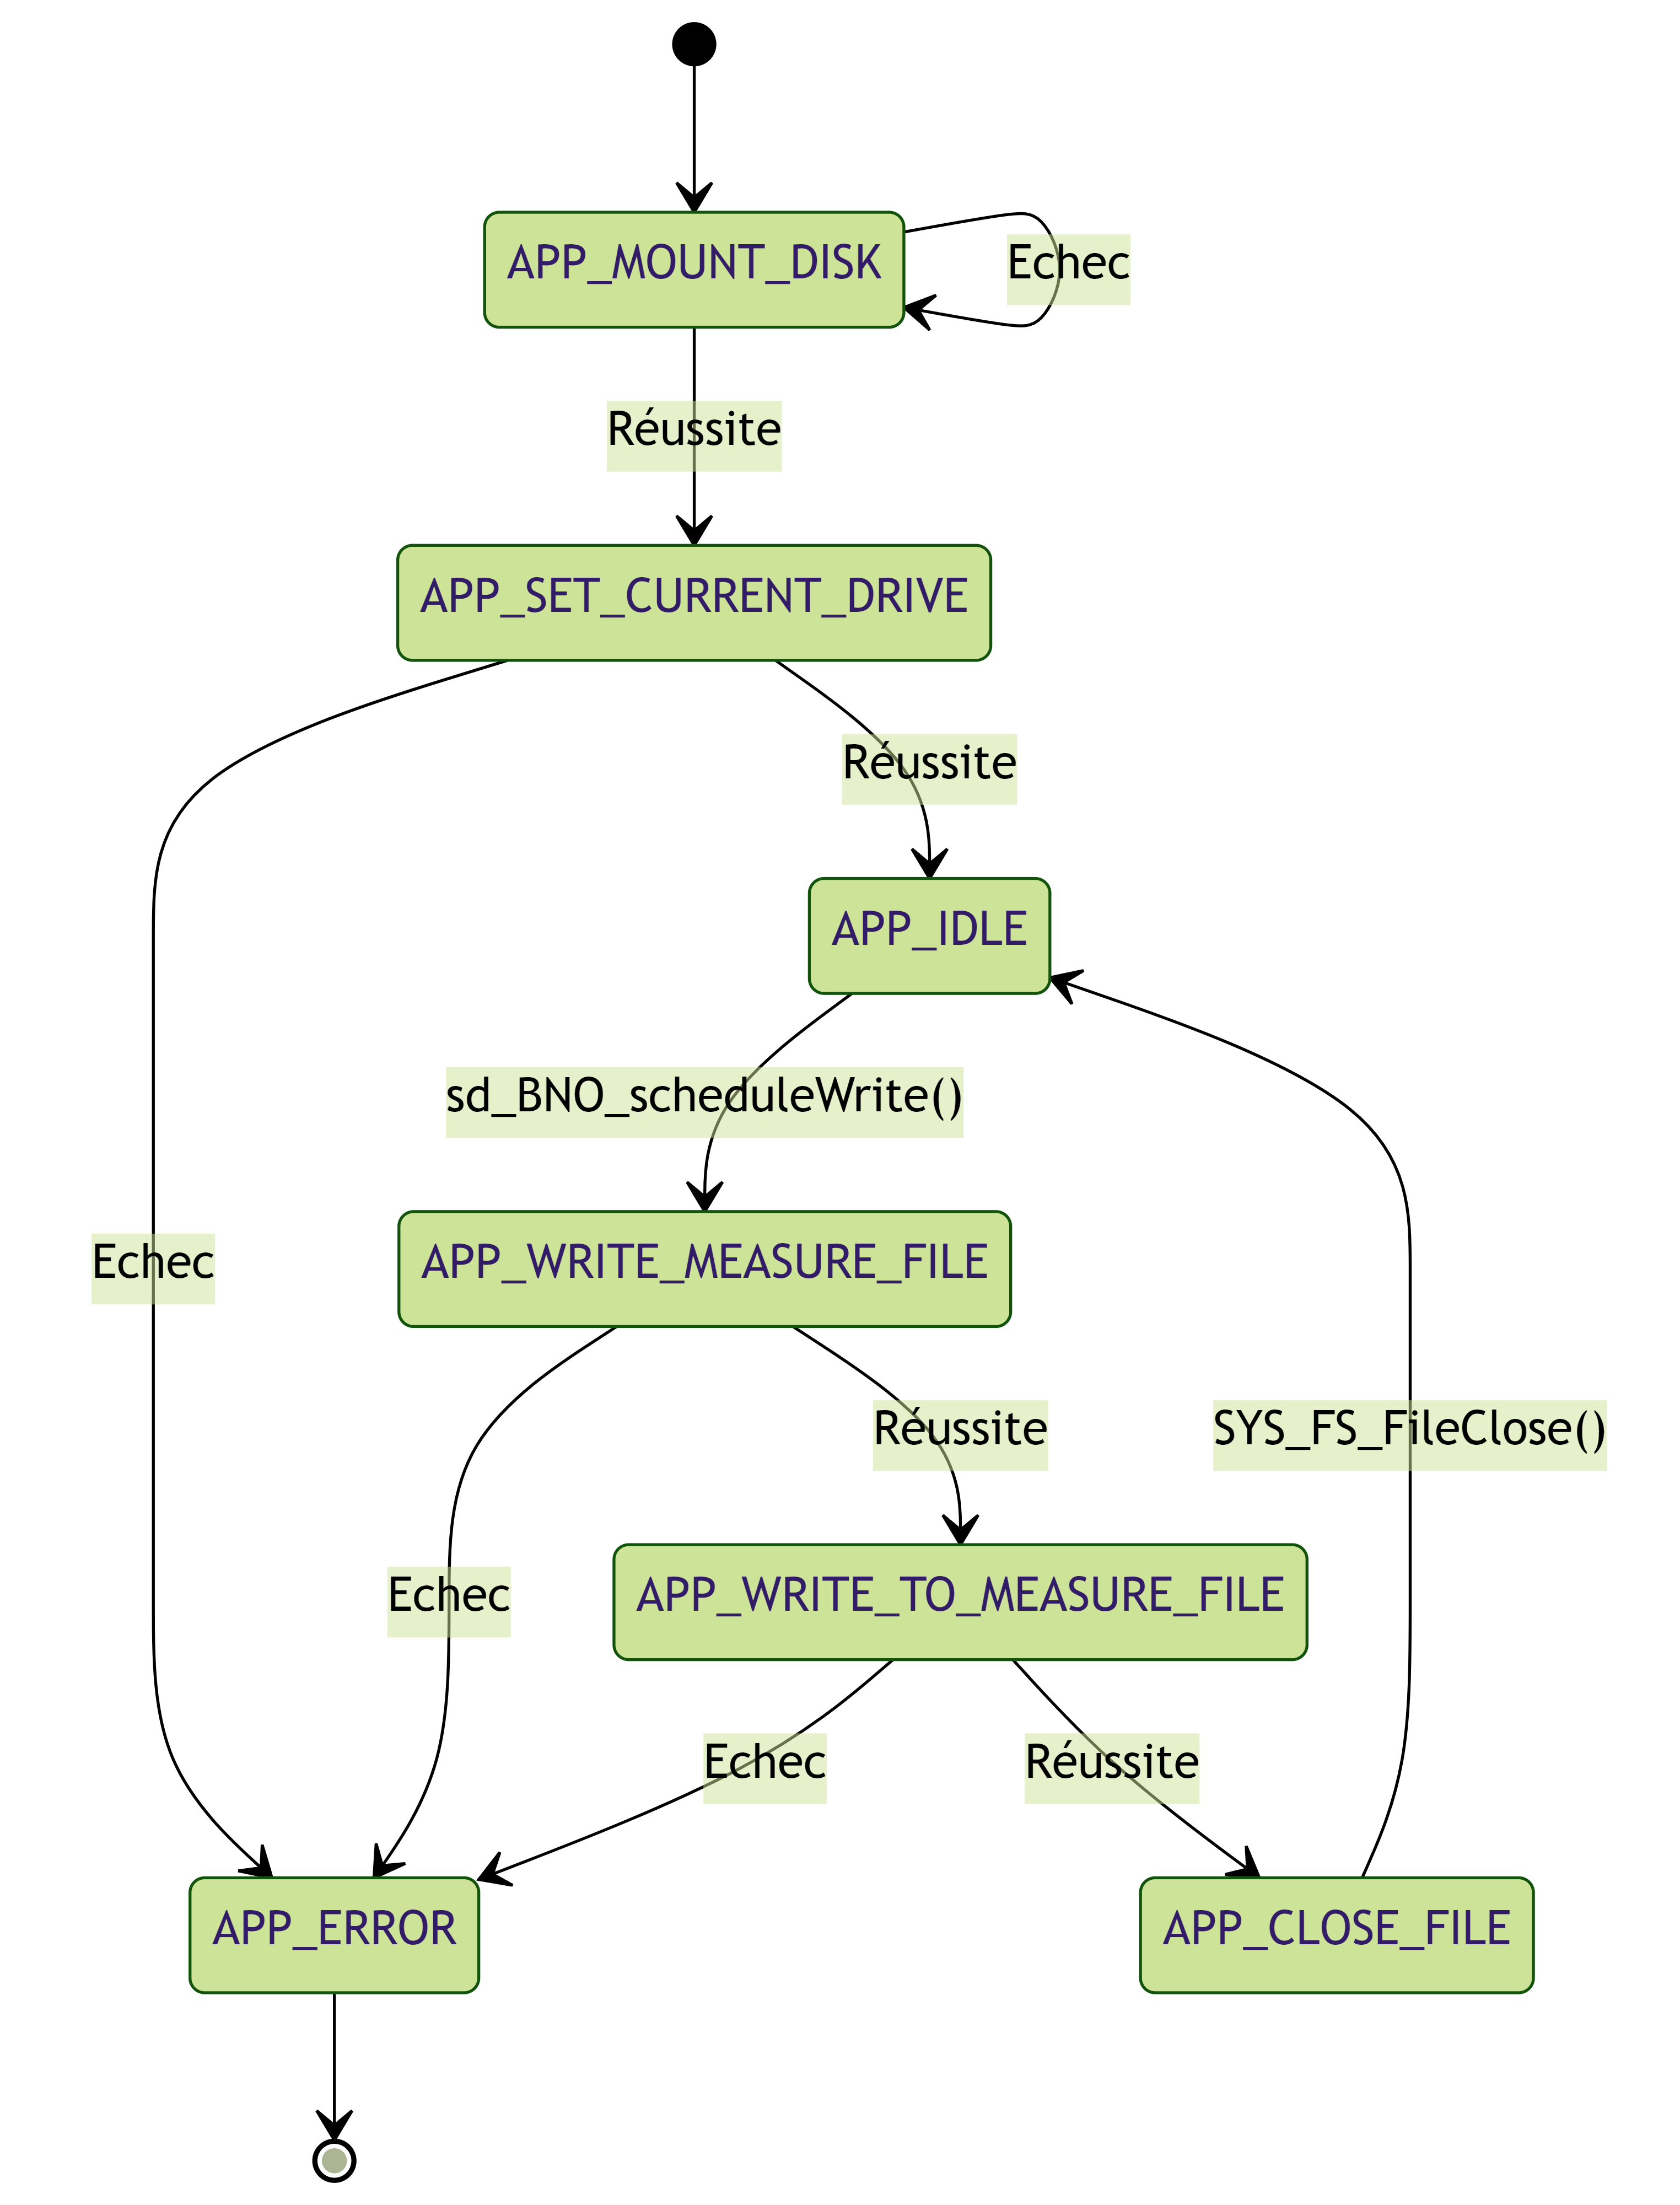
\includegraphics[width=0.6\linewidth]{Figures/Dev-SOFT/mermaid-diagram-2023-06-14-162436}
		\caption{Machine d'état de la carte SD}
		\label{fig:mermaid-diagram-2023-06-14-162436}
	\end{figure}

	\clearpage
	
	\paragraph{Planification d'une écriture}
	Afin de lancer une écriture d'un set de mesure sur la carte SD, il faut utiliser la fonction \textit{sd\_BNO\_scheduleWrite()} qui vas préparer le buffer d'écriture et modifier l'état de la carte SD : 
	\begin{lstlisting}[frame=single, language=C, caption={Lancement d'une écriture sur la carte SD}, captionpos=b, breaklines=true]
/* Write measures to sdCard */
sd_BNO_scheduleWrite(&bno055_local_data);
	\end{lstlisting}
	
	
	
	
	
	
	
	
	\clearpage
	

}
